\documentclass[tikz,border=2pt]{standalone}
\usepackage{amsmath,amssymb}
\usepackage{tikz}

\begin{document}
% Two metrics are topologically equivalent when every ball of one contains, around each of
% its points, a ball of the other (and vice versa): they then declare the same sets open.
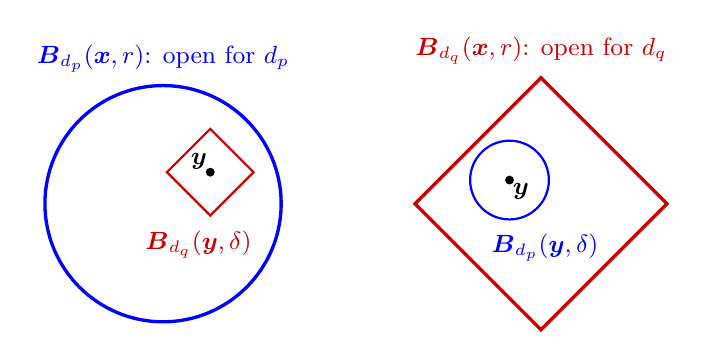
\begin{tikzpicture}[every node/.style={font=\small}]
	\draw[blue, very thick] (0,0) circle (1.5);
	\fill (0.6,0.4) circle (1.6pt) node[above left, inner sep=1pt] {$\boldsymbol{y}$};
	\draw[red!80!black, thick] (1.15,0.4) -- (0.6,0.95) -- (0.05,0.4) -- (0.6,-0.15) -- cycle;
	\node[blue, anchor=south] at (0,1.55) {$\boldsymbol{B}_{d_p}(\boldsymbol{x},r)$: open for $d_p$};
	\node[red!80!black, anchor=north] at (0.45,-0.22) {$\boldsymbol{B}_{d_q}(\boldsymbol{y},\delta)$};
	\begin{scope}[xshift=4.8cm]
		\draw[red!80!black, very thick] (1.6,0) -- (0,1.6) -- (-1.6,0) -- (0,-1.6) -- cycle;
		\fill (-0.4,0.3) circle (1.6pt) node[below right, inner sep=1pt] {$\boldsymbol{y}$};
		\draw[blue, thick] (-0.4,0.3) circle (0.5);
		\node[red!80!black, anchor=south] at (0,1.65) {$\boldsymbol{B}_{d_q}(\boldsymbol{x},r)$: open for $d_q$};
		\node[blue, anchor=north] at (0.05,-0.26) {$\boldsymbol{B}_{d_p}(\boldsymbol{y},\delta)$};
	\end{scope}
\end{tikzpicture}
\end{document}
